%%%%%%%%%%%%%%%%%%%%%%%%%%%%%%%%%%%%%%%%%%%%%%%%%%%%%%%%%%%%
\section{SB08 -- Comparative (Homology) Modelling \done}

\subsection*{Table of Contents}

\begin{enumerate}
\item Protein structure prediction
\item Principles of homology modelling
\item Template identification
\item Sequence alignment
\item Model building
\item Loop modelling
\item Side-chain modelling
\item Model refinement
\item Model validation and quality assessment
\item Limitations of comparative modelling
\end{enumerate}


\subsection*{Possible Exam Questions:}

\begin{enumerate}
\item{\textcolor{blue}{Describe the main steps involved in homology (comparative) modelling.} \done}
\item{Why is sequence alignment the most critical step? \done}
\item{Explain the difference between \textit{fragment-based} and \textit{restraint-based} raw model building. \done}
\item{How are side chains modelled? \done}
\item{How is model quality evaluated? \done}
\item{What are the main limitations of comparative modelling? \done}
\end{enumerate}


\paragraph{Describe the main steps involved in homology (comparative) modelling.}
Homology modelling is the method of predicting the structure of a protein (“target”) based on
experimentally determined structures of other proteins (“templates”). Main steps:

\begin{enumerate}
\item template identification: search databases for homologous proteins with known
structures;
\item sequence alignment: align target and template. 
\item building raw model: for aligned regions, backbone coordinates of the template are
directly copied to the target model;
\item loop modelling: coordinates for the variable regions (e.g. loops) and positions near
indels must be predicted.
\item side chains refinement: the side chains of the target sequence are added to the
backbone model, and their positioning is optimised to reduce steric clashes;
\item model plausibility assessment: stereochemical checks (e.g. bond lengths, angles,
Ramachandran plot), detection of steric clashes, computation of knowledge-based
scoring functions (statistical potentials) for comparison with experimentally observed
structures.
\end{enumerate}

\paragraph{Why is sequence alignment the most critical step in the homology modelling pipeline?}
Often, the best sequence alignment (the one that maximizes alignment score) is not optimal for structure modelling. Suboptimal choices at this stage cannot be corrected in the following steps. This makes the sequence alignment the most critical step in homology modelling.


\paragraph{Explain the difference between fragment-based and restraint-based raw model building.}
In comparative modelling, once the target-template alignment has been obtained, the raw model can be built using different strategies.

\noindent In fragment-based building, useful structural fragments are directly copied from one or more templates and assembled into the target model. The main advantage is that the copied fragments already have realistic local geometry, so important regions such as an active site can be preserved accurately. However, different fragments must then be joined together, and this may create problems in the global consistency of the model.

\noindent In restraint-based building, instead of copying entire fragments, the template is used to derive geometrical restraints on the target structure, for example approximate atomic positions, distances, or angles. The model is then obtained by optimizing the structure so that these restraints are satisfied as well as possible. This produces a globally optimized structure and spreads errors over the whole model, but it does not necessarily preserve the exact local geometry of specific functional regions.

\paragraph{How are side chains modelled?}

Side chains are usually modelled after the backbone has been constructed. Their conformations are mainly determined by rotations around single bonds, described by the side-chain torsion angles $\chi$. These angles do not take arbitrary values, but tend to adopt a small number of preferred conformations called \textbf{rotamers}. For each torsion angle, the main preferred positions are:
gauche$^+$, around $60^\circ$, gauche$^-$, around $-60^\circ$, and trans, around $180^\circ$.
\begin{center}
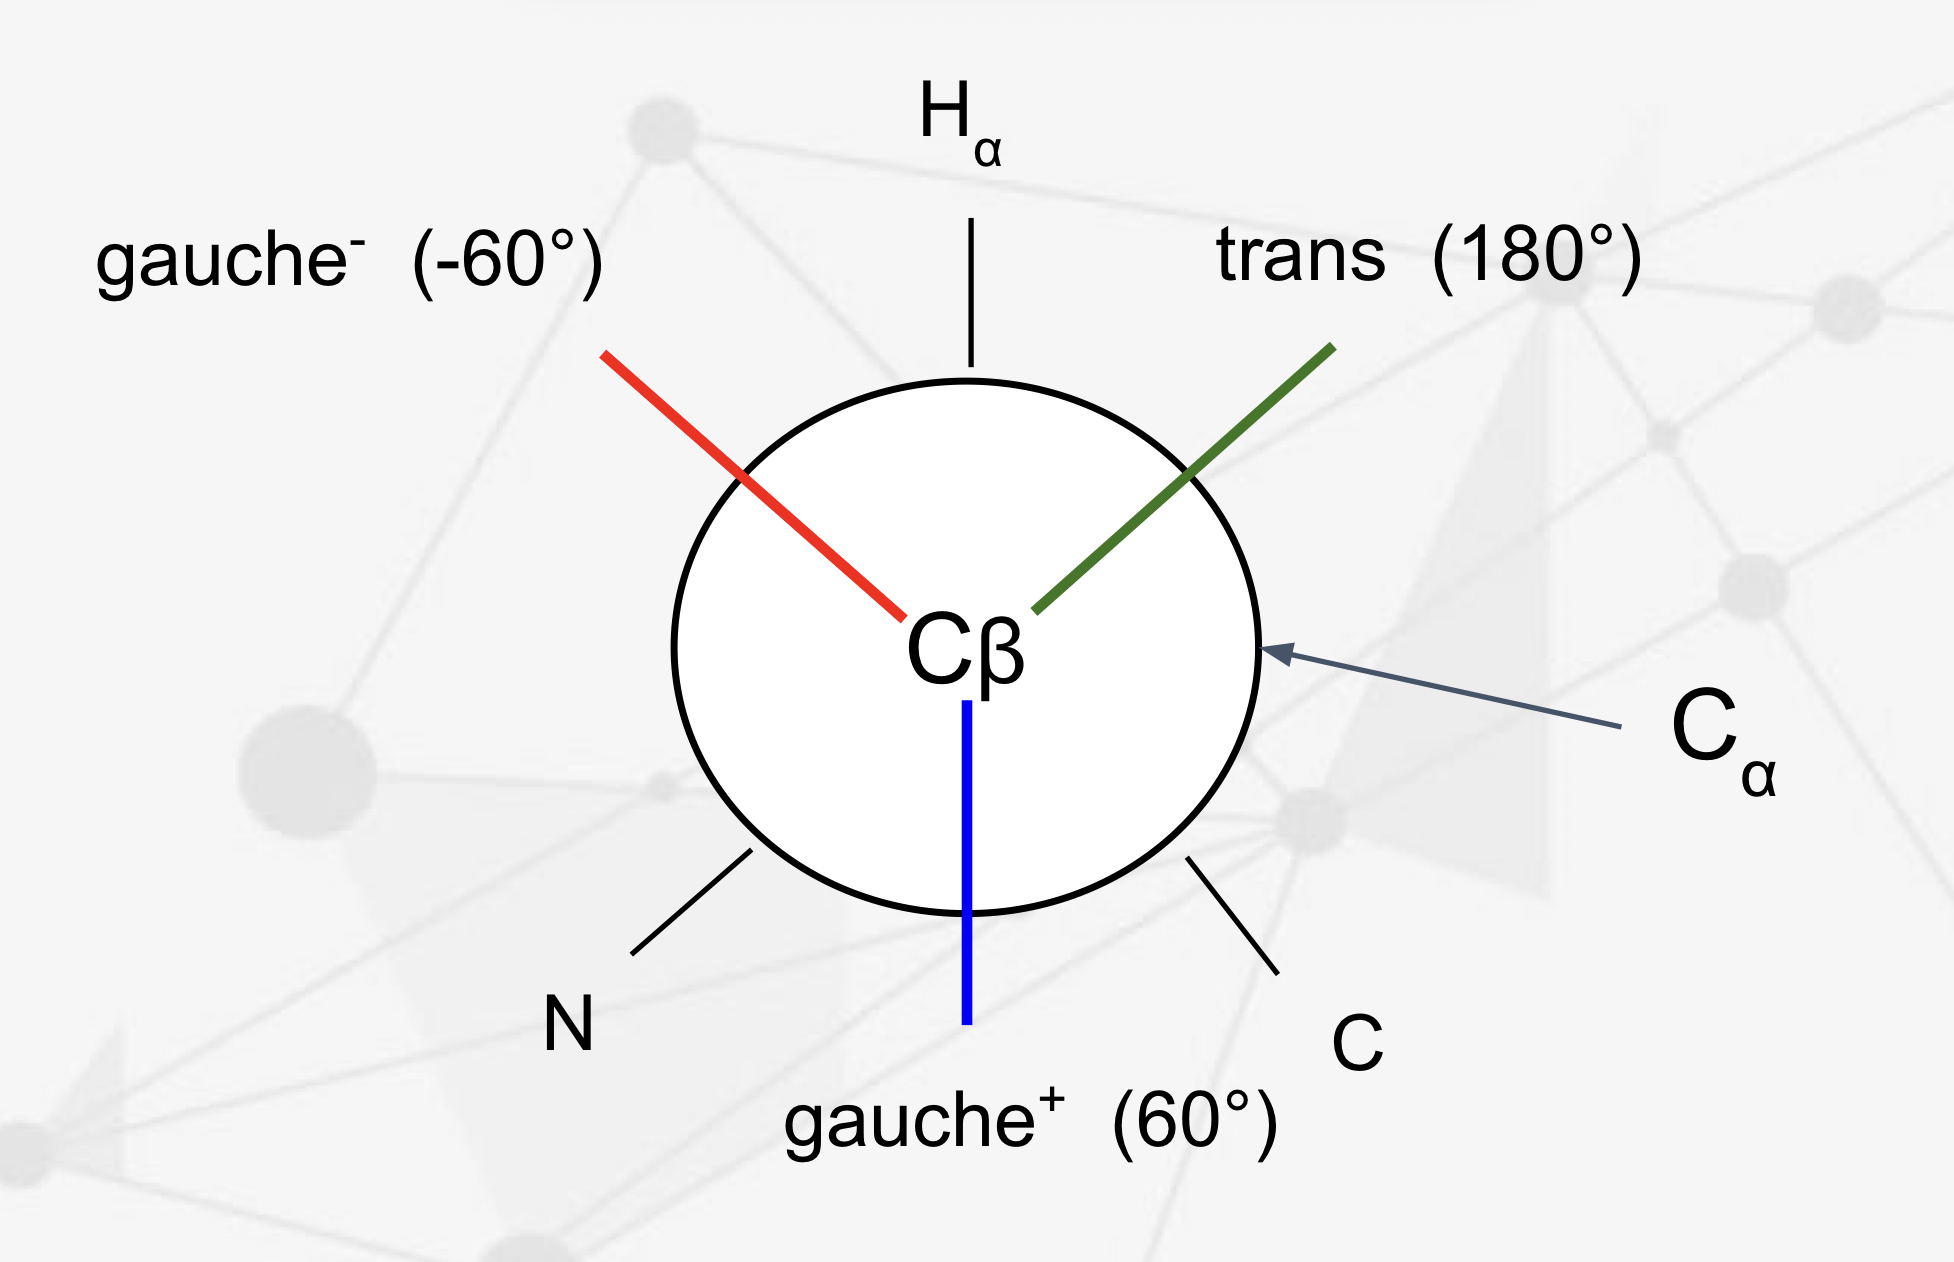
\includegraphics[width=0.4\textwidth]{figures/rotameters.png}
\end{center}
In homology modelling, side chains are therefore modelled by choosing suitable rotamers from a rotamer library. The probability of each rotamer depends on the type of amino acid and on the local backbone conformation, especially the backbone torsion angles $\phi$ and $\psi$. Side-chain modelling is not independent residue by residue, because the conformation chosen for one side chain can affect neighbouring residues through steric clashes and packing interactions. This creates a domino effect. When possible, it is preferable to keep the conformation of the template side chains, especially in conserved or functionally important regions, because they may already represent a realistic local geometry.

\paragraph{How is model quality assessed?}
The quality of a homology model is assessed by checking both its stereochemical correctness and its compatibility with known protein structures. First, one looks for \textbf{steric clashes}, where atoms are unrealistically close to each other. A good model should not contain severe overlaps between atoms. Second, one checks the \textbf{standard geometry} of the model, such as bond lengths, bond angles, peptide planarity, and backbone torsion angles. For example, the $\phi$ and $\psi$ angles should mostly fall in allowed regions of the Ramachandran plot.

A further level of assessment uses \textbf{statistical potentials} or frequency profiles. These methods compare the local environment of each residue with what is commonly observed in experimentally solved protein structures. For example, hydrophobic residues are expected to be buried, polar residues are often exposed, and certain residue types prefer specific secondary-structure or packing environments. If many residues are found in unusual environments, this suggests that the model may be unreliable.


\paragraph{What are the main limitations of comparative modelling?}
The main limitations of comparative modelling are i) the fact that the model will be more precise in regions that are conserved between the target and the template, and less accurate in variable regions such as loops; ii) that
you need homologous templates with known structures, which may not be available for all target sequences. In fact, $40\%$ of known genes are not homologous to known structures. This strongly limits the applicability  of homology modelling.